\documentclass[12pt]{article}

\usepackage[utf8]{inputenc}
\usepackage[T1]{fontenc}
\usepackage{babel}
\usepackage{lmodern}
\usepackage{geometry}
\geometry{margin=1in}
\usepackage{setspace}
\onehalfspacing
\usepackage{amsmath,amssymb}
\usepackage{booktabs}
\usepackage{graphicx}
\usepackage{float}
\usepackage{caption}
\usepackage{subcaption}
\usepackage{hyperref}
\usepackage{natbib}

\hypersetup{
  colorlinks=true,
  linkcolor=blue,
  citecolor=blue,
  urlcolor=blue,
  pdftitle={Espiral salario-precios en Paraguay},
  pdfauthor={Diego Bernardo Meza}
}

% Auto-generated by scripts/generate_assets.py
\newcommand\nEventosTotal{23}
\newcommand\nEventosMain{22}
\newcommand\eiGeneralMain{-0.067}
\newcommand\eiAlimentosMain{-0.054}
\newcommand\pGeneralMain{0.581}
\newcommand\pAlimentosMain{0.835}


\title{Espiral Salario--Precios en Paraguay:\\
Evidencia Descriptiva y de Evento con Datos Laborales, de Hogares y de Inflacion}

\author{
Diego Bernardo Meza\\
\small Investigador independiente\\
\small \texttt{dmeza.py@gmail.com}
\and
Colaboracion metodologica con Diego Daniel Sanabria
}

\date{\today}

\begin{document}
\maketitle

\begin{abstract}
Este articulo analiza el fenomeno de espiral salario--precios para Paraguay integrando tres fuentes: microdatos laborales (R02), microdatos de hogares (R01) e inflacion mensual con hitos de ajuste del salario minimo legal (SML). Con una estrategia de evento de ventana simetrica, se identifican \nEventosTotal{} eventos con datos completos y \nEventosMain{} eventos no solapados en la especificacion principal (h = 6). El efecto de evento promedio sobre IPC general es \eiGeneralMain{} pp y sobre IPC alimentos es \eiAlimentosMain{} pp; los placebo Monte Carlo asociados arrojan p-valores de \pGeneralMain{} y \pAlimentosMain{}, respectivamente. Los resultados sugieren heterogeneidad temporal y sensibilidad a especificaciones, por lo que la evidencia se interpreta como insumo analitico para politica publica, no como prueba causal definitiva.
\end{abstract}

\noindent\textbf{Palabras clave:} salario minimo, inflacion, pass-through, formalidad, Paraguay.\\
\textbf{JEL:} J31, E31, C21.

\section{Introduccion}

La discusion sobre salario minimo suele enfocarse en empleo y salarios, pero una pregunta central para macro y politica social es el posible traspaso hacia precios (``espiral salario--precios''). En economias con alta heterogeneidad laboral e informalidad, la magnitud de ese traspaso puede variar entre periodos y canastas de consumo.

La literatura internacional documenta que el salario minimo puede generar ajustes de precios en rubros intensivos en trabajo de bajos salarios \citep{aaronson2008, cengiz2019}. Tambien muestra que los efectos distributivos y de formalizacion dependen del contexto institucional y de enforcement \citep{card1995, dube2019}. En este marco, Paraguay ofrece un caso relevante por la combinacion de reajustes discretos del SML, dinamica inflacionaria y cambios recientes en indicadores de hogares.

Este trabajo contribuye con una plataforma reproducible y un articulo tecnico centrado en cuatro objetivos:
\begin{enumerate}
  \item cuantificar diferencias pre/post de inflacion en ventanas alrededor de ajustes del SML;
  \item comparar esas diferencias con distribuciones placebo (Monte Carlo);
  \item integrar contexto laboral (R02) y de hogares (R01) para lectura economica de los hallazgos;
  \item documentar limites de interpretacion para uso responsable de evidencia en decision publica.
\end{enumerate}

El enfoque es deliberadamente transparente: todos los cuadros y figuras del articulo se generan desde scripts reproducibles incluidos en esta carpeta.

Como aporte aplicado para divulgacion y uso por tomadores de decision, el estudio se complementa con una app web interactiva del proyecto, disponible en \url{https://diegomezapy.github.io/estudioSMLparaguay/}.

\section{Datos y metodologia}

\subsection{Fuentes de datos}

Se integran tres bloques:
\begin{itemize}
  \item \textbf{R02 (EPHC personas):} ingresos laborales, formalidad y caracteristicas sociodemograficas.
  \item \textbf{R01 (EPHC hogares):} conectividad, calidad material de vivienda y movilidad del hogar.
  \item \textbf{Serie macro mensual:} IPC general, IPC alimentos y fechas de ajuste del salario minimo legal.
\end{itemize}

Los indicadores de hogares se agregan por trimestre y se unen con los de R02 via etiqueta temporal \texttt{YYYYTrimQ}. Para evitar comparaciones invalidas, se diferencia explicitamente entre unidad persona (R02) y unidad hogar (R01).

\subsection{Variables de interes}

\begin{itemize}
  \item \textbf{Franja salarial relativa al SML:} \texttt{Menos de 1 SML}, \texttt{1 SML}, \texttt{Mas de 1 SML}, con tolerancia base de $\pm 10\%$.
  \item \textbf{Formalidad laboral:} proxy de cotizacion a caja/IPS.
  \item \textbf{Indicadores R01:} porcentaje de hogares con internet, material habitacional apto y movilidad propia.
  \item \textbf{Inflacion mensual:} variacion porcentual del indice respecto al mes previo para IPC general y alimentos.
\end{itemize}

\subsection{Estrategia empirica de evento}

Para cada evento de ajuste del SML se construye una ventana simetrica de $h$ meses pre y post (especificacion principal: $h=6$). El estadistico principal es:
\begin{equation}
EI_e = \overline{\pi}^{\,post}_e - \overline{\pi}^{\,pre}_e,
\end{equation}
donde $\pi$ representa inflacion mensual y $e$ denota evento.

Se reporta ademas un indicador de traspaso acumulado:
\begin{equation}
CT_e = \frac{EI_e}{\Delta SML_e},
\end{equation}
con $\Delta SML_e$ en puntos porcentuales.

La inferencia descriptiva se complementa con placebo Monte Carlo: se sortean ventanas ``no-evento'' de igual tamano y se compara el $EI$ observado frente a la distribucion simulada.

\subsection{Configuracion principal}

La configuracion central del paper usa eventos no solapados y $h=6$, con \nEventosMain{} eventos. Los resultados clave se resumen en la Tabla~\ref{tab:key}.

\begin{table}[H]
\centering
\caption{Resultados clave de la especificacion principal}
\label{tab:key}
\begin{tabular}{lr}
\toprule
Indicador & Valor\\
\midrule
Eventos identificados (total) & 23.000\\
Eventos usados (h=6, no solapados) & 22.000\\
EI IPC general (pp) & -0.067\\
EI IPC alimentos (pp) & -0.054\\
CT general (EI/ajuste) & -0.003\\
CT alimentos (EI/ajuste) & 0.023\\
p-value placebo IPC general & 0.581\\
p-value placebo IPC alimentos & 0.835\\
\bottomrule
\end{tabular}

\end{table}

\section{Resultados}

\subsection{Perfil promedio del evento}

La Figura~\ref{fig:event} muestra la trayectoria promedio relativa al periodo pre-evento. Visualmente, el patron es heterogeneo: hay eventos con aumentos y eventos con caidas de inflacion post-ajuste.

\begin{figure}[H]
\centering
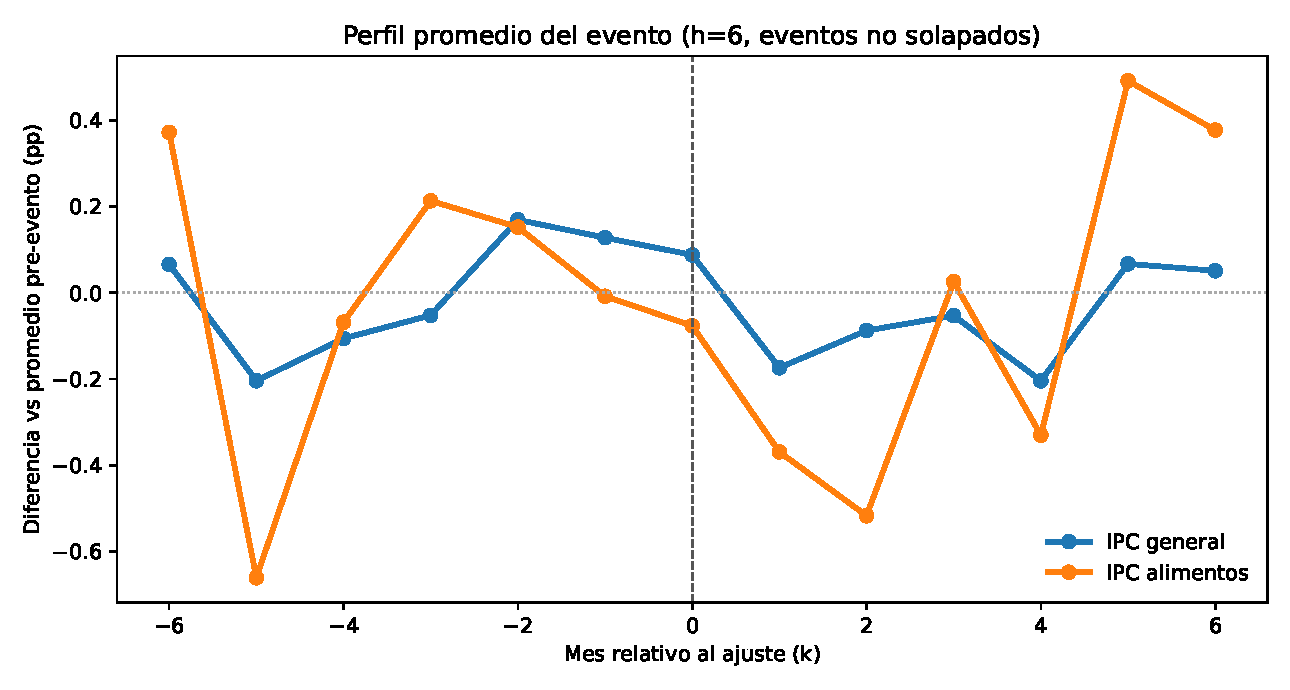
\includegraphics[width=0.92\textwidth]{figures/fig_event_profile.pdf}
\caption{Perfil promedio de inflacion alrededor del ajuste del SML (h=6, eventos no solapados)}
\label{fig:event}
\end{figure}

A nivel promedio, el EI en IPC general es \eiGeneralMain{} pp y en IPC alimentos \eiAlimentosMain{} pp.

\subsection{Evidencia placebo}

La Figura~\ref{fig:placebo} ubica el EI observado frente a su distribucion placebo. Los p-valores de referencia son \pGeneralMain{} para IPC general y \pAlimentosMain{} para IPC alimentos. Esto sugiere cautela frente a inferencias fuertes de causalidad en la especificacion principal.

\begin{figure}[H]
\centering
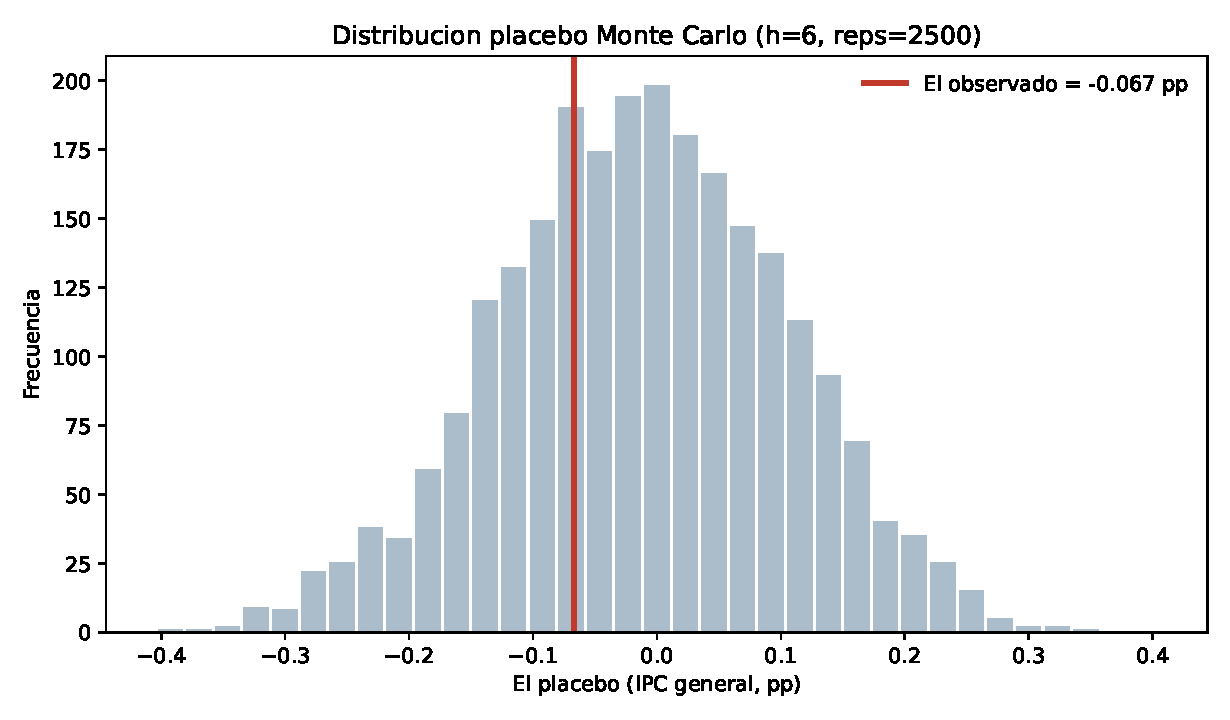
\includegraphics[width=0.85\textwidth]{figures/fig_placebo_hist.pdf}
\caption{Distribucion placebo Monte Carlo para EI de IPC general}
\label{fig:placebo}
\end{figure}

\subsection{Robustez de ventanas y limpieza de solapamiento}

La Tabla~\ref{tab:rob} resume sensibilidad por horizonte ($h=3,6,9$) y criterio de solapamiento. La magnitud y significancia descriptiva varian con la especificacion, consistente con shocks macro y composicion temporal de eventos.

\begin{table}[H]
\centering
\caption{Robustez por horizonte y criterio de solapamiento}
\label{tab:rob}
\begin{tabular}{rlrrrrr}
\toprule
h & Solap. & N & EI gen & EI alim & p gen & p alim\\
\midrule
3 & all & 24 & -0.269 & -0.500 & 0.095 & 0.178\\
3 & clean & 24 & -0.269 & -0.500 & 0.095 & 0.178\\
6 & all & 23 & -0.149 & -0.184 & 0.194 & 0.456\\
6 & clean & 22 & -0.067 & -0.054 & 0.579 & 0.821\\
9 & all & 22 & -0.042 & 0.036 & 0.613 & 0.842\\
9 & clean & 18 & 0.069 & 0.246 & 0.481 & 0.189\\
\bottomrule
\end{tabular}

\end{table}

\subsection{Contexto laboral y de hogares}

La Figura~\ref{fig:contexto} integra series trimestrales de R02 y R01 con marcas de trimestres de ajuste del SML. Esta lectura permite contextualizar el fenomeno en dinamicas de formalidad, conectividad y condiciones del hogar.

\begin{figure}[H]
\centering
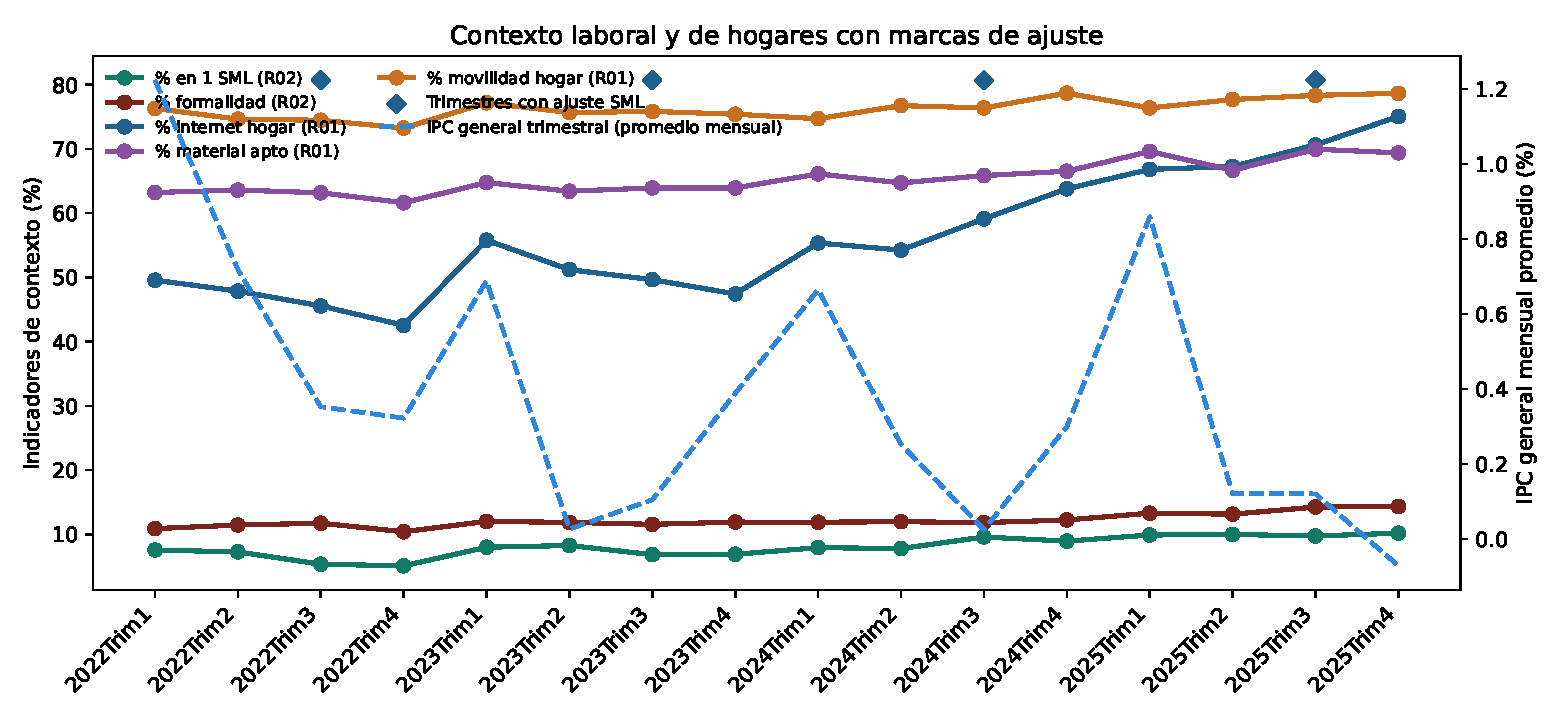
\includegraphics[width=0.98\textwidth]{figures/fig_contexto_trimestral.pdf}
\caption{Contexto R02 + R01 con marcas de trimestres de ajuste del SML}
\label{fig:contexto}
\end{figure}

Como complemento distributivo, la Figura~\ref{fig:densidad} muestra concentracion de masa alrededor de 1 SML (banda $\pm 10\%$), en linea con patrones de bunching descriptivo.

\begin{figure}[H]
\centering
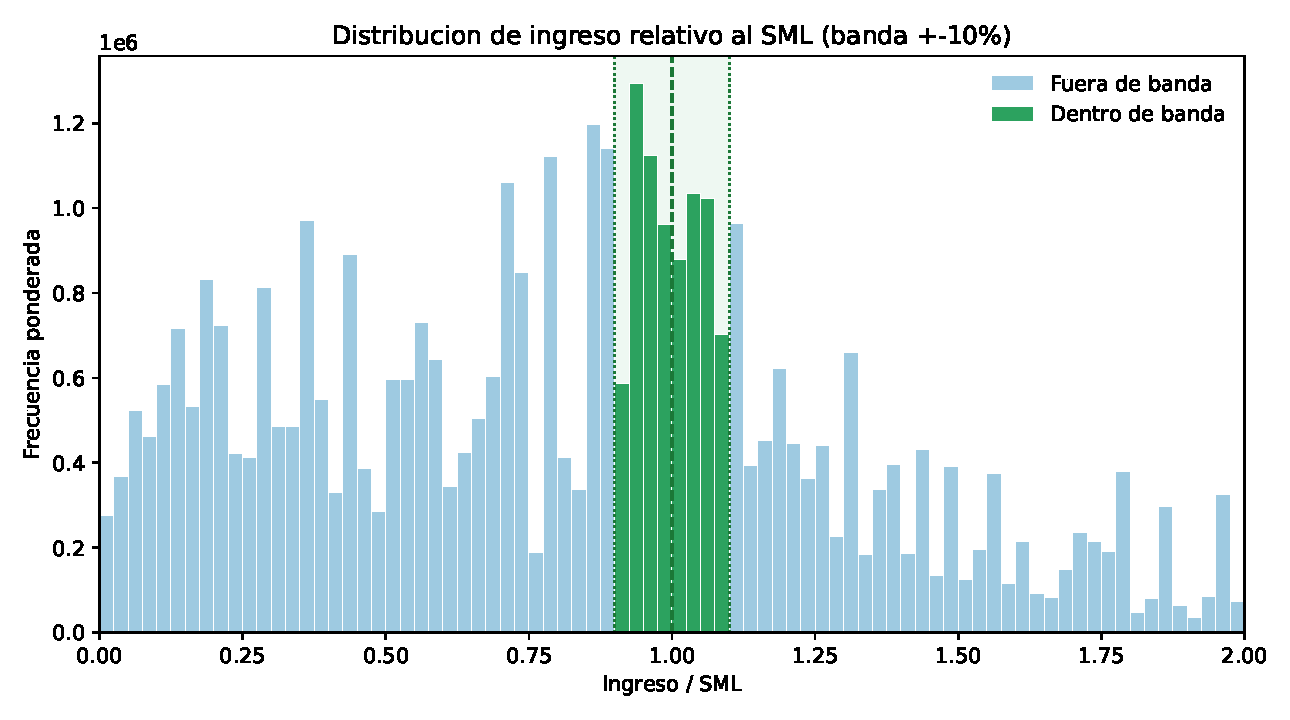
\includegraphics[width=0.86\textwidth]{figures/fig_density_rel_sml.pdf}
\caption{Distribucion de ingreso relativo al SML y banda $\pm 10\%$}
\label{fig:densidad}
\end{figure}

\subsection{Auditoria por evento}

Para trazabilidad, la Tabla~\ref{tab:eventos} reporta ajuste, EI y coeficientes de traspaso por evento individual.

\begin{table}[H]
\centering
\caption{Metricas por evento (especificacion principal)}
\label{tab:eventos}
\begin{tabular}{lrrrrr}
\toprule
Fecha & Ajuste (pp) & EI IPC gen & EI IPC alim & CT gen & CT alim\\
\midrule
1996-04-01 & 10.000 & -0.865 & -1.002 & -0.087 & -0.100\\
1997-01-01 & 10.000 & 0.509 & 0.716 & 0.051 & 0.072\\
1998-03-01 & 12.000 & 0.514 & 0.641 & 0.043 & 0.053\\
2000-02-01 & 15.000 & 0.026 & -0.365 & 0.002 & -0.024\\
2001-05-01 & 15.000 & -0.340 & -1.295 & -0.023 & -0.086\\
2002-08-01 & 12.000 & 0.621 & 2.072 & 0.052 & 0.173\\
2005-04-01 & 12.000 & 0.262 & 0.220 & 0.022 & 0.018\\
2006-04-01 & 12.000 & -0.672 & -1.513 & -0.056 & -0.126\\
2007-10-01 & 10.000 & -0.347 & -1.139 & -0.035 & -0.114\\
2009-05-01 & 5.000 & 0.385 & 1.334 & 0.077 & 0.267\\
2010-07-01 & 7.000 & 0.660 & 1.702 & 0.094 & 0.243\\
2011-04-01 & 10.000 & -1.480 & -3.870 & -0.148 & -0.387\\
2014-03-01 & 10.000 & -0.663 & -1.486 & -0.066 & -0.149\\
2016-12-01 & 7.700 & 0.239 & 0.413 & 0.031 & 0.054\\
2017-07-01 & 3.900 & 0.193 & 0.615 & 0.050 & 0.158\\
2018-07-01 & 3.500 & -0.053 & 0.374 & -0.015 & 0.107\\
2019-07-01 & 3.800 & -0.035 & 0.246 & -0.009 & 0.065\\
2021-07-01 & 4.400 & 0.664 & 1.848 & 0.151 & 0.420\\
2022-07-01 & 11.400 & -0.556 & -0.418 & -0.049 & -0.037\\
2023-07-01 & 5.100 & 0.043 & 0.589 & 0.008 & 0.116\\
2024-07-01 & 4.400 & -0.148 & -0.466 & -0.034 & -0.106\\
2025-07-01 & 3.600 & -0.430 & -0.398 & -0.119 & -0.111\\
\bottomrule
\end{tabular}

\end{table}

\begin{table}[H]
\centering
\caption{Contexto trimestral 2025 (R02 + R01)}
\label{tab:ctx2025}
\begin{tabular}{lrrrrr}
\toprule
Trimestre & \% 1 SML & \% formalidad & \% internet & \% material apto & \% movilidad\\
\midrule
2025Trim1 & 9.904 & 13.304 & 66.805 & 69.593 & 76.374\\
2025Trim2 & 9.994 & 13.146 & 67.259 & 66.671 & 77.682\\
2025Trim3 & 9.748 & 14.252 & 70.629 & 69.951 & 78.332\\
2025Trim4 & 10.193 & 14.357 & 75.042 & 69.378 & 78.649\\
\bottomrule
\end{tabular}

\end{table}

\section{Discusion e implicancias}

Los resultados no respaldan una narrativa unica de espiral sostenida en toda la muestra; mas bien, sugieren comportamiento dependiente de episodio y especificacion. Para politica publica, esto implica que la calibracion de reajustes del SML deberia evaluarse junto con:
\begin{itemize}
  \item composicion sectorial y de formalidad del empleo;
  \item dinamica de precios en alimentos frente a IPC general;
  \item condiciones de bienestar del hogar que afectan vulnerabilidad inflacionaria.
\end{itemize}

La evidencia de bunching alrededor de 1 SML y los diferenciales por contexto social abren agenda para estrategias complementarias: fiscalizacion laboral, politicas de productividad y focalizacion por hogares de alta exposicion.

\section{Conclusion}

Este articulo presenta una arquitectura reproducible para estudiar la relacion salario minimo--precios en Paraguay combinando evento, placebo y contexto micro. En la especificacion principal, los EI promedio son moderados (\eiGeneralMain{} pp en IPC general y \eiAlimentosMain{} pp en IPC alimentos) y estadisticamente fragiles frente a placebo. Por tanto, la contribucion principal es metodologica y de transparencia: proveer evidencia trazable, actualizable y util para dialogo tecnico.

\section*{Declaraciones para publicacion}

\paragraph{Contribucion y colaboracion metodologica.}
Implementacion del articulo y del sistema reproducible por Diego Bernardo Meza. La seccion metodologica se desarrolla en colaboracion con el enfoque original del estadistico Diego Daniel Sanabria.

\paragraph{Disponibilidad de datos y codigo.}
La carpeta incluye tablas y figuras listas para compilar en Overleaf. Tambien incluye el script \texttt{scripts/generate\_assets.py} para regenerar insumos a partir de los datos del proyecto principal. Como aporte complementario de transferencia y comunicacion de resultados, el tablero interactivo del estudio esta disponible en \url{https://diegomezapy.github.io/estudioSMLparaguay/}.

\paragraph{Limitaciones y uso responsable.}
Este trabajo ofrece evidencia descriptiva y de evento; no constituye por si mismo una identificacion causal estructural. Los resultados son sensibles a filtros, horizonte, criterio de solapamiento y calidad muestral de subgrupos.

\paragraph{Conflictos de interes.}
El autor declara no tener conflictos de interes financieros vinculados a este estudio.

\paragraph{Aprobacion etica.}
No se utilizan datos personales identificables; el analisis se basa en microdatos anonimizados y agregaciones estadisticas.


\bibliographystyle{apalike}
\bibliography{references}

\end{document}
